% !TEX encoding = UTF-8
% !TEX program = xelatex
\documentclass[12pt,a4paper]{article}
\usepackage[paperwidth=210mm, paperheight=297mm, left=0.75in, right=0.75in, bottom=1in, top=1in]{geometry}
\usepackage{polyglossia}
\setdefaultlanguage[babelshorthands]{italian}
\usepackage{fontspec}
\usepackage{graphicx}
\usepackage{blindtext}
\usepackage{wrapfig}

\frenchspacing
\makeindex

\begin{document}
\title{\vspace{-70pt}James Webb Space Telescope}
\author{Sebastiano Chiozzi}
\date{}
\maketitle
\pagestyle{empty}
\thispagestyle{empty}

\section*{Storia}
\label{storia}
\begin{wrapfigure}{r}{0.35\textwidth}
  \vspace{-10pt}
  \begin{center}
    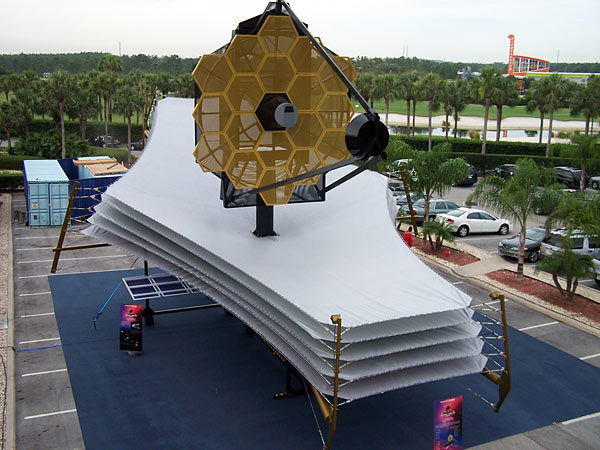
\includegraphics[width=0.30\textwidth]{satellite}
  \end{center}
  \vspace{-20pt}
\end{wrapfigure}
Il \textbf{Telescopio Spaziale James Webb (JWST)} è un telescopio spaziale sviluppato per diventare il successore del precedente \emph{Telescopio spaziale Hubble}, più precisamente nel campo dell'\textbf{osservazione infrarossa}. Verrà costruito e gestito, in cooperazione, dalla NASA, dall'Agenzia Spaziale Europea e dall'Agenzia Spaziale Canadese.

Precedentemente indicato come Next Generation Space Telescope (o NGST), è stato rinominato nel 2002 in onore del secondo amministratore della NASA James E. Webb.
Il suo lancio è previsto per il 2018.

JWST è stato sviluppato appositamente per migliorare notevolmente l'osservazione nello \emph{spettro infrarosso}, con l'obiettivo principale di osservare le galassie responsabili della ri-ionizzazione dell'universo primordiale e esaminare il residuo a infrarossi del big bang, in modo da poter determinare le condizioni iniziali di \emph{formazione dell'universo}.

\section*{Osservazioni}
\label{osservazioni}

Il telescopio sarà dotato di \textbf{sensori} estremamente sensibili e sarà posizionato in un'orbita molto più elevata rispetto a Hubble, a circa 1,5 milioni di chilometri dal sistema Terra-Luna. Tale posizione infatti, offre la massima sensibilità alla radiazione infrarossa. Inoltre, la maggior parte delle interferenze infrarosse (provenienti proprio dal Sole, dalla Terra e dalla Luna) verranno bloccate grazie ad un'\textbf{ampia paratia} metallizzata utilizzata come schermo.

La necessità di porre JWST in un un'orbita tanto elevata renderà virtualmente \emph{impossibile qualunque missione di manutenzione o aggiornamento}. Non si tratta di un limite di poco conto, vista l'importanza che tali missioni hanno avuto per il telescopio Hubble che nel tempo è stato più volte riparato e aggiornato, sostituendo via via quasi tutti gli strumenti ottici. Proprio per questo motivo i test a terra sono maniacali e hanno portato a un sempre continuo \emph{aumento dei costi di realizzazione}.

\section*{Curiosità}
\label{curiosit}

Nel giugno 2011, è stato riferito che il telescopio Webb costerà almeno quattro volte di più rispetto a quanto originariamente proposto.
Alcuni scienziati hanno espresso preoccupazione per i crescenti costi e ritardi di pianificazione del progetto.

\end{document}